\bframe{Accomplishments}
\begin{itemize}
\item Boundary integral method (Xin, Lucas)
\item Bending model with area area-difference elasticity (Xin)
\item Yin-Yang model for red cell (Xin)
\item Curvature estimation for volume-of-fluid (Petr)
\item Simulations of membrane-less electrochemical reactor (Petr)
\item Multi-marker volume-of-fluid (Petr)
\item Neutral network for curvature (Petr)
\item Bayesian inference for red cell (Athena, George, Lucas)
\item Inertial focusing of spherical particles (Dmitry, Athena, Lucas)
\end{itemize}
\eframe

\bframe{Highlights}
\begin{itemize}
\item Adaptive resolution
%\item Boundary condition for particle method
\begin{center}
  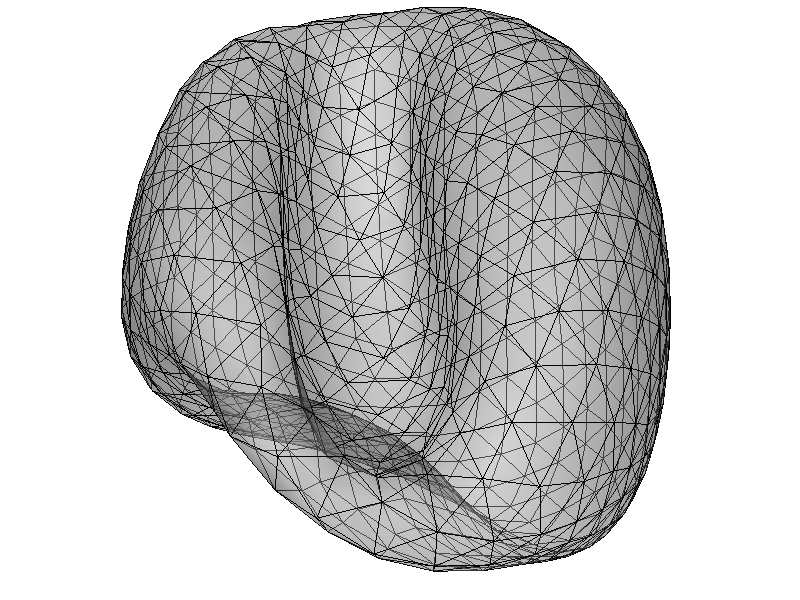
\includegraphics[width=0.5\textwidth]{i/b.png}
\end{center}
\begin{center}
  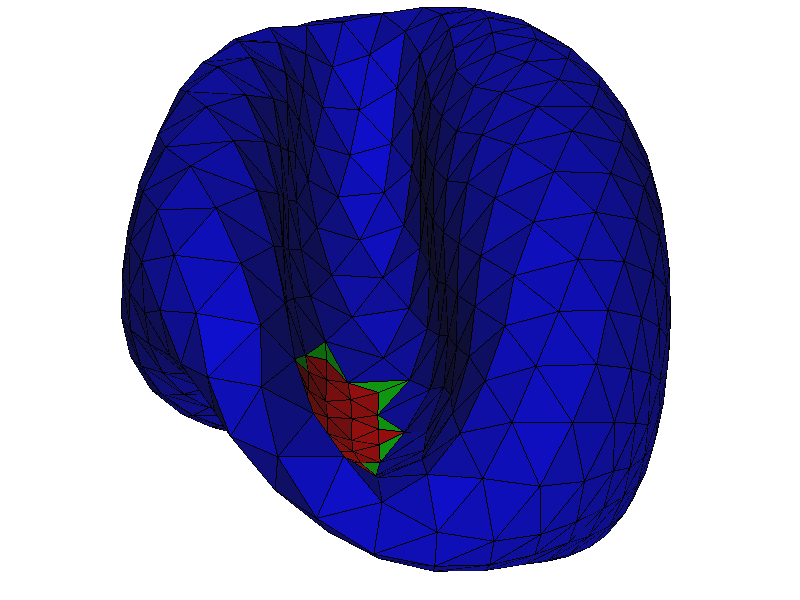
\includegraphics[width=0.5\textwidth]{i/a.png}
\end{center}
\end{itemize}
\eframe

\bframe{Most interesting}
- Yin and Yang (Xin)
\eframe
